% import gaya yang sudah disiapkan
\documentclass{gaya}

% import berbagai variabel
\titleind{Tolok Ukur LLM: Panduan untuk Mengevaluasi Model Bahasa} % yang ini untuk di cover
\titleindinline{LLM Benchmarks: Guide to Evaluating Language Models} % yang ini untuk di dalam paragraf
\titleen{LLM Benchmarks: Guide to Evaluating Language Models}

\fullname{Budi Kesana Kemari} % diisi nama Anda
\newcommand{\fullnamenc}{Budi Kesana Kemari} % diisi nama Anda
\idnum{120450081} % diisi NIM Anda

\approvaldate{06 April 2024} % diisi tanggal penulisan
\newcommand{\approvaldatenc}{06 April 2024}

\degre{Sarjana Sains Data}
\yearsubmit{2024} % diisi tahun penulisan
\program{Sains Data} % prodi
\dept{Sains} % fakultas

\firstsupervisor{Prof. Dr. Mantab Selalu, M.Si.} % nama pembimbing 1
\nipnrkfirst{NIP. } % diisi NIP atau NRK
\firstnip{194508171980031002}

\secondsupervisor{Bimbing Baik Hati, S.Si., M.Si.} % nama pembimbing 2
\nipnrksecond{NRK. }
\secondnip{199008172020031003}

\firstexaminer{Penguji 1} % nama penguji 1
\secondexaminer{Penguji 2} % nama penguji 2

\headofdepartment{Dr. Kaprodi Kami, M.Sc.} % nama koordinator prodi
\nipnrkhead{NRK. }
\headnip{199102302020012003}

\def\tahapan{sidang} % opsi: sempro, semhas, sidang, atau final

%-----------------------------------------------
% Input tahapan Tugas akhir Anda saat ini
%-----------------------------------------------
% diisi dengan:
% sempro (jika dibuat untuk seminar proposal),
% semhas (jika untuk seminar hasil),
% sidang (untuk sidang), atau
% final (jika sudah final dan siap cetak)

\def\sempro{sempro}
\def\semhas{semhas}
\def\sidang{sidang}
\def\final{final}

\ifx\tahapan\sempro
\textta{Proposal Skripsi}
\textoncover{Diajukan sebagai syarat maju seminar proposal}
\textonapproval{Naskah Proposal Tugas Akhir } \else
\ifx\tahapan\semhas
\textta{Naskah Skripsi}
\textoncover{Diajukan sebagai syarat maju seminar hasil}
\textonapproval{Naskah Tugas Akhir untuk Seminar Hasil } \else
\ifx\tahapan\sidang
\textta{Naskah Skripsi}
\textoncover{Diajukan sebagai syarat maju sidang tugas akhir}
\textonapproval{Naskah Skripsi untuk Sidang Akhir } \else
\ifx\tahapan\final
\textta{Skripsi}
\textoncover{Diajukan sebagai syarat untuk memperoleh gelar Sarjana}
\textonapproval{Tugas Akhir Sarjana } \else
\textta{SALAH INPUT!!!}
\textoncover{SALAH INPUT!!!}
\textonaproval{SALAH INPUT!!!}
\fi
\fi
\fi
\fi


% pemenggalan kata
% Hyphenation untuk Indonesia 
% @author  Ridlo Wahyudi Wibowo (+Kikun)
% 
% Tambahkan cara pemenggalan kata-kata yang salah dipenggal secara otomatis 
% oleh LaTeX. Jika kata tersebut dapat dipenggal dengan benar, maka tidak 
% perlu ditambahkan dalam berkas ini. Tanda pemenggalan kata menggunakan 
% tanda '-'; contoh:
% menarik
%   --> pemenggalan: me-na-rik
%
% selalu baca ulang dokumen untuk menemukan pemenggalan yang kurang tepat setelah pemenggalan 
% lain diperbaiki
\hyphenation{
    %spesial
    % alphabhet A
    a-na-li-sa
    a-tur 
    a-pli-ka-si 
    at-mos-fer
    ak-si
    ada-lah
    arc-se-cond
    % alphabhet B
    bumi
    ba-ngun-an 
    be-be-ra-pa 
    ber-in-ter-ak-si
    be-ru-pa
    be-ra-gam
    ber-ge-rak
    ber-ke-lan-jut-an 
    ber-pe-nga-ruh 
    ber-dasar-kan
    % alphabhet C
    ca-ri
    count
    cit-ra
    % alphabhet D
    di-sim-pan di-pim-pin de-ngan da-e-rah di-ba-ngun da-pat di-nya-ta-kan 
    di-sim-bol-kan di-pi-lih di-li-hat de-fi-ni-si
    di-ban-ding-kan
    di-si-mu-la-si-kan
    di-li-bat-kan
    di-se-bab-kan
    di-la-ku-kan
    di-je-las-kan
    di-tambah-kan
    di-temu-kan
    di-masuk-kan
    di-gu-na-kan
    di-ka-te-go-ri-kan
    di-ber-da-ya-kan
    di-a-frag-ma
    di-ha-sil-kan
    di-trans-for-ma-si
    di-bu-tuh-kan
    di-uta-ma-kan
    % alphabhet E
    e-ner-gi eks-klu-sif
    error
    equa-tor
    % alphabhet F
    fa-si-li-tas
    fitting
    fo-to-me-tri
    front-side
    for-mat-kan
    % alphabhet G
    ga-bung-an ge-rak
    % alphabhet H
    ha-lang-an
    % alphabhet I
    im-age
%    institut
    % alphabhet J
    % alphabhet K
    ke-hi-lang-an
	ke-sta-bil-an
    ku-ning 
    kua-li-tas ka-me-ra 
    ke-mung-kin-an 
    ke-se-pa-ham-an
    ko-e-fi-si-en
    kupang
    ko-or-di-nat
    % alphabhet L
    LINEAR
    ling-kung-an
    % alphabhet M
    mat-riks
    me-neng-ah
    meng-a-tas-i me-mung-kin-kan me-nge-na-i me-ngi-rim-kan 
    meng-u-bah meng-a-dap-ta-si me-nya-ta-kan mo-di-fi-ka-si
    meng-a-tur
    meng-gu-na-kan
		meng-ha-sil-kan
		me-nam-bah-kan
		me-nen-tu-kan
    me-nun-juk-kan
    meng-hu-bung-kan
    mem-per-li-hat-kan		
    me-man-fa-at-kan
    men-je-las-kan
    me-nye-bab-kan
    me-ru-pa-kan
    me-li-bat-kan
    meng-a-ki-bat-kan
    mengajari
    mengelilingi
    me-ning-kat-kan
    mem-be-ri-kan
    mul-ti-vari-ate
    me-mub-li-ka-si-kan
    % alphabhet N
    nya-ta non-eks-klu-sif
    ni-lai-nya
    non-eks-klu-sif
    % alphabhet O
    neo-wise
    ob-ser-va-to-ri-um
    ob-ser-va-tions
    % alphabhet P
    pack-age
    pro-grade
	pe-nye-rap-an 
	pe-ngon-trol
    pe-mo-del-an
    pe-ran  pe-ran-an-nya
    pem-ba-ngun-an 
    pre-si-den 
    pe-me-rin-tah 
    prio-ri-tas 
    peng-am-bil-an
    pen-di-di-kan
    peng-ga-bung-an
    pe-nga-was-an 
    pe-ngem-bang-an 
    pe-nga-ruh 
    pa-ra-lel-is-me 
    pe-rin-tah
    per-hi-tung-an 
    per-ma-sa-lah-an 
    pen-ca-ri-an 
    peng-struk-tur-an
    per-ban-ding-an
    per-kuliah-an
    pub-li-ka-si
    pe-nga-ta-log-an
    pe-nu-lis
    pen-cip-ta
    po-si-tion-ing
    pub-lish-ing
    pub-li-ca-tions
    % alphabhet Q
    % alphabhet R
    range
    ran-cang-an
    re-tro-grade
    % alphabhet S
    si-mu-la-si sa-ngat sur-vey sur-vei
    se-dang-kan
    stag-nan
    stan-dar-di-sa-si
	sub-sti-tu-si
    sub-bab
    sains
    skrip-si
    spec-tro-pho-to-me-tric
    sci-ence
    soft-ware
    % alphabhet T
    te-ngah
    ter-da-pat
    tisserand
	tri-angu-lar
    trans-for-ma-si
    Tilong
    terbuka
    % alphabhet U
    % alphabhet V
    % alphabhet W
    with
    % alphabhet X
    % alphabhet Y
    % alphabhet Z
    % special
    % < 3 huruf dan 1 huruf penggalan
    itu ini aku kau di si ke bui ibu tua tai tau ras pos ban dan cat cap cek cor akan alam asam ikan iring orang oli ubah ulang udang arang api elang amin aman iba 
    % asing
    log-book
}

% Isi keseluruhan dokumen
\begin{document}

% Sampul luar bahasa indonesia
\cover
\newpage

% Nomor halaman pembuka dimulai dari sini
\pagenumbering{roman}

% Sampul dalam bahasa indonesia
\coverdalam
\newpage

% Halaman pengesahan
\approvalpage
\cleardoublepage

% Halaman orisinalitas
\originalitypage
\cleardoublepage

% Halaman publikasi
\publicationpage
\cleardoublepage

% Abstrak Bahasa Indonesia
\begin{abstractind}
\justifying

Lorem ipsum dolor sit amet, consectetur adipisicing elit, sed do eiusmod tempor incididunt ut labore et dolore magna aliqua. Ut enim ad minim veniam, quis nostrud exercitation ullamco laboris nisi ut aliquip ex ea commodo consequat. Duis aute irure dolor in reprehenderit in voluptate velit esse cillum dolore eu fugiat nulla pariatur. Excepteur sint occaecat cupidatat non proident, sunt in culpa qui officia deserunt mollit anim id est laborum. Sed ut perspiciatis unde omnis iste natus error sit voluptatem accusantium doloremque laudantium, totam rem aperiam, eaque ipsa quae ab illo inventore veritatis et quasi architecto beatae vitae dicta sunt explicabo. Nemo enim ipsam voluptatem quia voluptas sit aspernatur aut odit aut fugit, sed quia consequuntur magni dolores eos qui ratione voluptatem sequi nesciunt.
%%pada abstrak bahasa Inggris, separator desimal koma

\bigskip
\noindent
\textbf{Kata kunci:} ini, itu, ini, itu % masukkan keyword
\end{abstractind}

\cleardoublepage

% Abstrak Bahasa Inggris
\begin{abstracteng}
\justifying
\emph{
Lorem ipsum dolor sit amet, consectetur adipisicing elit, sed do eiusmod tempor incididunt ut labore et dolore magna aliqua. Ut enim ad minim veniam, quis nostrud exercitation ullamco laboris nisi ut aliquip ex ea commodo consequat. Duis aute irure dolor in reprehenderit in voluptate velit esse cillum dolore eu fugiat nulla pariatur. Excepteur sint occaecat cupidatat non proident, sunt in culpa qui officia deserunt mollit anim id est laborum. Sed ut perspiciatis unde omnis iste natus error sit voluptatem accusantium doloremque laudantium, totam rem aperiam, eaque ipsa quae ab illo inventore veritatis et quasi architecto beatae vitae dicta sunt explicabo. Nemo enim ipsam voluptatem quia voluptas sit aspernatur aut odit aut fugit, sed quia consequuntur magni dolores eos qui ratione voluptatem sequi nesciunt.}
%%pada abstrak bahasa Inggris, separator desimal titik

\bigskip
\noindent
\textbf{\emph{Keywords :}} \emph{this, that, this, thatthis}.
\end{abstracteng}

\cleardoublepage

% Motto
\motto
\begin{centering}
\vfill
\emph{Ini mottoku, mana motto-mu?.\\[.6cm]}
\vfill
\end{centering}

\cleardoublepage

% Persembahan
\acknowledgment
\begin{centering}
\vfill
\emph{Untuk Emak dan Bapak\\di kampung\\[.5cm]}
\vfill
\end{centering}

\cleardoublepage

% Kata pengantar
%-----------------------------------------------------------------
%Di sini awal masukan untuk Prakata
%-----------------------------------------------------------------
\preface
\justifying
\noindent Puji syukur penulis panjatkan ke hadirat Allah SWT atas berkah dan rahmat-Nya sehingga skripsi ini dapat terselesaikan dengan baik. Skripsi ini dibuat untuk menyelesaikan pendidikan jenjang sarjana pada Institut Teknologi Sumatera. Penyusunan skripsi ini banyak mendapat bantuan dan dukungan dari berbagai pihak sehingga dalam kesempatan ini, dengan penuh kerendahan hati, penulis mengucapkan terima kasih kepada:

\begin{enumerate}
\item{Prof. Xxxx Xxxx selaku  Rektor Institut Teknologi Sumatera,}
\item{Prof. Yyyy Yyyy selaku Dekan Fakultas Sains Institut Teknologi Sumatera,}
\item{Dr. Zzzz Zzzz selaku Koordinator Program Studi,}
\item{Prof. Dr. Nama selaku dosen pembimbing pertama yang telah membimbing,}
\item{Nama , S.Si., M.Si. selaku dosen pembimbing kedua yang selalu membantu, dan }
\item{Cantumkan pihak-pihak lain yang membantu penelitian tugas akhir, termasuk sumber data, tempat riset, rekan satu TA, dan-lain-lain.}
\end{enumerate}

Penulis menyadari bahwa penyusunan Skripsi ini jauh dari sempurna.
Akhir kata penulis mohon maaf yang sebesar-besarnya apabila ada kekeliruan di dalam penulisan skripsi ini.


\vspace{0.5cm}

\begin{flushright}
\begin{tabular}{p{3.5cm}l}
&Lampung Selatan, \approvaldatenc \\[1.5cm]
&\textbf{\fullnamenc}
\end{tabular}
\end{flushright}

\cleardoublepage

% Daftar Isi
\addcontentsline{toc}{chapter}{DAFTAR ISI}
\tableofcontents

% Daftar Gambar
\phantomsection%<---
\addcontentsline{toc}{chapter}{DAFTAR GAMBAR}
\listoffigures

% Daftar Tabel
\phantomsection%<---
\addcontentsline{toc}{chapter}{DAFTAR TABEL}
\listoftables

%% Daftar Singkatan
%\singkatan

\begin{flushleft}\vspace{0.5cm}
\begin{tabular}{p{1.5cm}p{2pt}l}
\textbf{A}\\
ADU & & Analog to Digital Units\\

\vspace{0.1cm}

\textbf{B}\\
BBU & & Belahan Bumi Utara\\
\vspace{0.1cm}

\textbf{C}\\
CCD & & Charge-Coupled Device\\
\vspace{0.1cm}

\textbf{M}\\
MPSAS & & Magnitude per Square Arcsecond\\
\vspace{0.1cm}

\textbf{N}\\
NOAO & & National Optical Astronomy Observatories\\
\vspace{0.1cm}


\end{tabular}
\end{flushleft}

%
%% Daftar Simbol
%\simbol

\begin{flushleft}\vspace{0.5cm}
\begin{tabular}{p{.5cm}p{2pt}l}
     $m_x$ &  & Magnitudo\\
     $F_x$ &  & Fluks\\
     $\phi_x$ & & Tegangan pada \emph{clock cycle} CCD\\
     $k$ & & Ekstingsi\\
     $\epsilon$ & & Koefisien transformasi magnitudo $v$ ke $V$ \\


\end{tabular}
\end{flushleft}


\newpage

% Nomor halaman isi dimulai dari sini
\pagenumbering{arabic}

% Bab 1 pendahuluan
\chapter{PENDAHULUAN}
\section{Latar Belakang}
\label{section:latarbelakang}
Bagian ini mendeskripsikan gambaran umum, konteks, dan posisi penelitian skripsi dalam konstelasi perkembangan pengetahuan yang telah dicapai. Penjelasan yang dituliskan menjadi penting karena dengan landasan yang kuat, maka pekerjaan penelitian yang lebih terarah dapat dilakukan. Hal ini lebih spesifik dan tegas disampaikan pada sub-sub bab berikutnya.

Beberapa pustaka utama yang berperan dominan dapat disampaikan di sini untuk memberi gambaran tentang letak penelitian TA dalam konstelasi keilmuan yang dicapai. Hasil-hasil dari pustaka terbaru dapat menopang Latar Belakang ini menjadi lebih kuat. Sangat wajar apabila isi sub bab setelah Latar Belakang ini mengalami penyesuaian saat sejumlah hasil penelitian sudah diperoleh dan dianalisis. Oleh karena itu, finalisasi isi Pendahuluan ini biasanya dilakukan menjelang akhir pembuatan laporan penelitian yang dituangkan dalam skripsi \cite{malasan_photometric_1986, malasan_remote_2006}.

\section{Rumusan Masalah}
Bagian ini menjadi salah satu bagian penting dalam Pendahuluan. Setelah paparan Latar Belakang \ref{section:latarbelakang}, maka masalah yang diangkat pada pekerjaan penelitian perlu dirumuskan dengan baik. Pertanyaan apa yang akan dijawab dalam penelitian dapat ditulis dalam kalimat tanya ataupun tidak.

Berdasarkan latar belakang yang telah dijelaskan sebelumnya, berikut merupakan rumusan masalah pada penelitian tugas akhir ini:
\begin{enumerate}
    \item Bagaimana curah hujan berhubungan dengan tingkat pendapatan masyarakat?
    \item Apakah Candi Borobudur dibangun dengan mengikuti kaidah astronomi?
\end{enumerate}

\section{Tujuan Penelitian}
Eros reprimique vim no. Alii legendos volutpat in sed, sit enim nemore labores no. No odio decore causae has. Vim te falli libris neglegentur, eam in tempor delectus dignissim, nam hinc dictas an.

Tujuan dari penelitian ini berdasarkan rumusan masalah yang juga menjadi dasar dilakukannya penelitian ini adalah sebagai berikut:
\begin{enumerate}
    \item Melihat hubungan curah hujan dengan tingkat pendapatan masyarakat dengan metode blabla?
    \item Melakukan simulasi langit malam di masa Candi Borobudur dibangun?
\end{enumerate}

\section{Batasan Masalah}
Setiap masalah dan penelitian yang diangkat selalu memiliki batasan. Ada batasan, asumsi, atau kriteria yang menjadi pembatas atas masalah yang diangkat dalam penelitian TA, sehingga arah penelitian dapat fokus. Batasan ini perlu dituliskan secara tegas, dan dapat saja memuat lebih dari satu. Contoh batasan masalah misalnya batasan penggunaan data, area, rentang waktu, dan lain-lain.

% Sub bab lain dapat ditambahkan, misalnya:
%\section{Manfaat Penelitian}
%\section{Hipotesis}

% Bab 2 tinjauan pustaka
\chapter{TINJAUAN PUSTAKA}
% contoh opsi lain Bab 2
%\chapter{DASAR TEORI}


\section{Menulis Subbab dan Indentasi Paragraf}
Tulis subbab yang sesuai dengan penelitian yang dilakukan. Jumlah Subbab disesuaikan dengan penelitian sehingga cerita yang dibangun dan analisis yang ditulis lebih mudah untuk dipahami. Tulis referensi yang selengkap-lengkapnya dan menggambarkan perkembangan penelitian terkait.

Pro omnium incorrupte ea. Elitr eirmod ei qui, ex partem causae disputationi nec. Amet dicant no vis, eum modo omnes quaeque ad, antiopam evertitur reprehendunt pro ut. Nulla inermis est ne. Choro insolens mel ne, eos labitur nusquam eu, nec deserunt reformidans ut. His etiam copiosae principes te, sit brute atqui definiebas id \cite{mumpuni_future_2018}. Elitr eirmod ei qui, ex partem causae disputationi nec. Amet dicant no vis, eum modo omnes quaeque ad, antiopam evertitur reprehendunt pro ut. Nulla inermis est ne. Choro insolens mel ne, eos labitur nusquam eu, nec deserunt reformidans ut. His etiam copiosae principes te, sit brute atqui definiebas id.

Sit et labitur albucius elaboraret. Ceteros efficiantur mei ad. Hendrerit vulputate democritum est at, quem veniam ne has, mea te malis ignota volumus. Eros reprimique vim no. Alii legendos volutpat in sed, sit enim nemore labores no. No odio decore causae has. Vim te falli libris neglegentur, eam in tempor delectus dignissim, nam hinc dictas an. Sit et labitur albucius elaboraret. Ceteros efficiantur mei ad. Hendrerit vulputate democritum est at, quem veniam ne has, mea te malis ignota volumus. Eros reprimique vim no. Alii legendos volutpat in sed, sit enim nemore labores no. No odio decore causae has. Vim te falli libris neglegentur, eam in tempor delectus dignissim, nam hinc dictas an.

\subsection{Menulis Subsubbab}
Tulis Subsub bab jika diperlukan, dan harus lebih dari satu. Jika hanya satu bahasan maka tidak perlu dijadikan subsubbab. Begitu juga ketika menulis item, tidak perlu dijadikan item jika isinya hanya satu item.
\begin{enumerate}
    \item Ne per tota mollis suscipit. Ullum labitur vim ut, ea dicit eleifend dissentias sit. Duis praesent expetenda ne sed.
    \item Sit et labitur albucius elaboraret. Ceteros efficiantur mei ad.
    \item Hendrerit vulputate democritum est at, quem veniam ne has, mea te malis ignota volumus.
\end{enumerate}

Eros reprimique vim no. Alii legendos volutpat in sed, sit enim nemore labores no. No odio decore causae has. Vim te falli libris neglegentur, eam in tempor delectus dignissim, nam hinc dictas an. Ne per tota mollis suscipit. Ullum labitur vim ut, ea dicit eleifend dissentias sit. Duis praesent expetenda ne sed. Sit et labitur albucius elaboraret. Ceteros efficiantur mei ad. Hendrerit vulputate democritum est at, quem veniam ne has, mea te malis ignota volumus. Eros reprimique vim no. Alii legendos volutpat in sed, sit enim nemore labores no. No odio decore causae has. Vim te falli libris neglegentur, eam in tempor delectus dignissim, nam hinc dictas an.

Terkadang item ditulis tanpa penomoran, hal ini dilakukan untuk menunjukkan sesuatu yang jumlahnya tidak diketahui secara pasti. Penulisan item yang tidak bernomor contohnya adalah sebagai berikut:
\begin{itemize}
    \item Pro omnium incorrupte ea. Elitr eirmod ei qui, ex partem causae disputationi nec. Amet dicant
    \item No vis, eum modo omnes quaeque ad, antiopam evertitur reprehendunt pro ut.
    \item Nulla inermis est ne. Choro insolens mel ne, eos labitur nusquam eu, nec deserunt reformidans ut. His etiam copiosae principes te, sit brute atqui definiebas id.
\end{itemize}

Terkadang item penomoran ingin diubah sesuai format tertentu. Contohnya adalah sebagai berikut:
\begin{enumerate}[a).]
    \item Pro omnium incorrupte ea. Elitr eirmod ei qui, ex partem causae disputationi nec. Amet dicant
    \item No vis, eum modo omnes quaeque ad, antiopam evertitur reprehendunt pro ut.
    \item Nulla inermis est ne. Choro insolens mel ne, eos labitur nusquam eu, nec deserunt reformidans ut. His etiam copiosae principes te, sit brute atqui definiebas id.
\end{enumerate}

Terkadang item penomoran ingin diubah sesuai format tertentu. Contohnya adalah sebagai berikut:
\begin{itemize}
    \item[!!] Pro omnium incorrupte ea. Elitr eirmod ei qui, ex partem causae disputationi nec. Amet dicant
    \item[*] No vis, eum modo omnes quaeque ad, antiopam evertitur reprehendunt pro ut.
    \item[Step 1.] Nulla inermis est ne. Choro insolens mel ne, eos labitur nusquam eu, nec deserunt reformidans ut. His etiam copiosae principes te, sit brute atqui definiebas id.
\end{itemize}


\subsubsection{Menulis Subsubsubbab}
Ne per tota mollis suscipit. Ullum labitur vim ut, ea dicit eleifend dissentias sit. Duis praesent expetenda ne sed. Sit et labitur albucius elaboraret. Ceteros efficiantur mei ad. Hendrerit vulputate democritum est at, quem veniam ne has, mea te malis ignota volumus. Eros reprimique vim no. Alii legendos volutpat in sed, sit enim nemore labores no. No odio decore causae has. Vim te falli libris neglegentur, eam in tempor delectus dignissim, nam hinc dictas an.

\subsubsection{Contoh subsubsubbab lainnya}
Pro omnium incorrupte ea. Elitr eirmod ei qui, ex partem causae disputationi nec. Amet dicant no vis, eum modo omnes quaeque ad, antiopam evertitur reprehendunt pro ut. Nulla inermis est ne. Choro insolens mel ne, eos labitur nusquam eu, nec deserunt reformidans ut. His etiam copiosae principes te, sit brute atqui definiebas id.



\section{Menulis Persamaan}
Persamaan matematis dapat ditulis dalam berbagai bentuk. Beberapa faktor yang mempengaruhi penulisan antara lain: (1) apakah persamaan tadi perlu diberi nomor atau tidak (2) apakah ada persamaan-persamaan tadi dalam sebuah kelompok (3) atau apakah merupakan bentuk penurunan yang perlu disejajarkan (4) selain itu bisa juga persamaan yang ditulis di dalam teks.
\begin{equation}
E=mc^2
\end{equation}
    dengan $E$ adalah energi, $m$ adalah massa, dan $c$ adalah kecepatan cahaya.

\begin{equation}
\sqrt{x^2+1}
\end{equation}
    dengan $x$ adalah variabel.


\subsection{Persamaan inline}
Quo no atqui omnesque intellegat, ne nominavi argumentum quo. Eum ei purto oporteat dissentiet, soleat utamur an sit. Et assum dicam interpretaris quo. Cetero alterum ea vel, no possit alterum utroque nec. His fuisset quaestio ad. Has eu tritani incorrupte consequuntur, esse aliquip nec ne.


% Bab 3 metodologi penelitian
\chapter{METODE PENELITIAN}

\section{Isi Metode Penelitian}
Alat dan bahan yang digunakan pada penelitian ini terbagi atas perangkat keras dan perangkat lunak yang akan dijelaskan seperti berikut.

\section{Data}
Pro omnium incorrupte ea. Elitr eirmod ei qui, ex partem causae disputationi nec. Amet dicant no vis, eum modo omnes quaeque ad, antiopam evertitur reprehendunt pro ut. Nulla inermis est ne. Choro insolens mel ne, eos labitur nusquam eu, nec deserunt reformidans ut. His etiam copiosae principes te, sit brute atqui definiebas id.

\section{Alat dan Bahan}
Pro omnium incorrupte ea. Elitr eirmod ei qui, ex partem causae disputationi nec. Amet dicant no vis, eum modo omnes quaeque ad, antiopam evertitur reprehendunt pro ut. Nulla inermis est ne. Choro insolens mel ne, eos labitur nusquam eu, nec deserunt reformidans ut. His etiam copiosae principes te, sit brute atqui definiebas id.

    \subsection{Perangkat Keras}
    Pro omnium incorrupte ea. Elitr eirmod ei qui, ex partem causae disputationi nec. Amet dicant no vis, eum modo omnes quaeque ad, antiopam evertitur reprehendunt pro ut. Nulla inermis est ne. Choro insolens mel ne, eos labitur nusquam eu, nec deserunt reformidans ut. His etiam copiosae principes, teleskop yang bagus.

	\subsection{Perangkat Lunak}
    Pro omnium incorrupte ea. Elitr eirmod ei qui, ex partem causae disputationi nec. Amet dicant no vis, eum modo omnes quaeque ad, antiopam evertitur reprehendunt pro ut. Nulla inermis est ne. Choro insolens mel ne, eos labitur nusquam eu, nec deserunt reformidans ut. His etiam copiosae principes te, sit brute atqui definiebas id.
		\begin{enumerate}[a.]
		\itemsep0em
			\item Arduino IDE for Windows,
			\item IRAF,
		\end{enumerate}

\section{Alur Penelitian}
	Consul graeco signiferumque qui id, usu eu summo dicunt voluptatum, nec ne simul perpetua posidonium. Eos ea saepe prodesset signiferumque. No dolore possit est. Mei no justo intellegebat definitiones, vis ferri lorem eripuit ad. Solum tritani scribentur duo ei, his an adipisci intellegat.

\section{Tahapan Pelaksanaan}
	Consul graeco signiferumque qui id, usu eu summo dicunt voluptatum, nec ne simul perpetua posidonium. Eos ea saepe prodesset signiferumque. No dolore possit est. Mei no justo intellegebat definitiones, vis ferri lorem eripuit ad. Solum tritani scribentur duo ei, his an adipisci intellegat.

\section{Jadwal Kegiatan}
	Quo no atqui omnesque intellegat, ne nominavi argumentum quo. Eum ei purto oporteat dissentiet, soleat utamur an sit. Et assum dicam interpretaris quo. Cetero alterum ea vel, no possit alterum utroque nec. His fuisset quaestio ad. Has eu tritani incorrupte consequuntur, esse aliquip nec ne \ref{jadwal}.


	%Format tabel ini hanya untuk jadwal kegiatan saja
	%Bisa dibuat dulu di https://www.tablesgenerator.com/ baru dikopi ke dokumen ini
		\begin{table}[H]
		\centering
		\caption{Jadwal Penelitian.} % caption pakai titik?
		\label{jadwal}
		\begin{tabular}{|c|l|l|l|l|l|l|l|}
		\hline
		\multirow{2}{*}{No} & \multirow{2}{*}{Keterangan} & \multicolumn{6}{c|}{Bulan}                                                                                                                          \\ \cline{3-8}
		                    &                             & 1 & 2 & 3 & 4 & 5 & 6 \\ \hline
		1                   & Studi literatur                                  &\cellcolor{gray} &\cellcolor{gray}&                        &                        &                        &                         \\ \hline
		2                   & Desain                                           &                        &\cellcolor{gray}&\cellcolor{gray}&                        &                        &                         \\ \hline
		3                   & Pembelian bahan                                  &                        &                        &\cellcolor{gray}&                        &                        &                         \\ \hline
		4                   & Pembuatan prototipe                              &                        &                        &\cellcolor{gray}&\cellcolor{gray}&\cellcolor{gray}&                         \\ \hline
		5                   & Uji coba dan perbaikan                           &                        &                        &                        &\cellcolor{gray}&\cellcolor{gray}&                         \\ \hline
		6                   & Penulisan tugas akhir                               &                        &                        &                        &                        &                        &\cellcolor{gray}\\ \hline
		\end{tabular}
		\end{table}


\section{Melampirkan Gambar}
Pro omnium incorrupte ea. Elitr eirmod ei qui, ex partem causae disputationi nec. Amet dicant no vis, eum modo omnes quaeque ad, antiopam evertitur reprehendunt pro ut. Nulla inermis est ne. Choro insolens mel ne, eos labitur nusquam eu, nec deserunt reformidans ut. His etiam copiosae principes te, sit brute atqui definiebas id.

\begin{figure}[H]
    \centering
    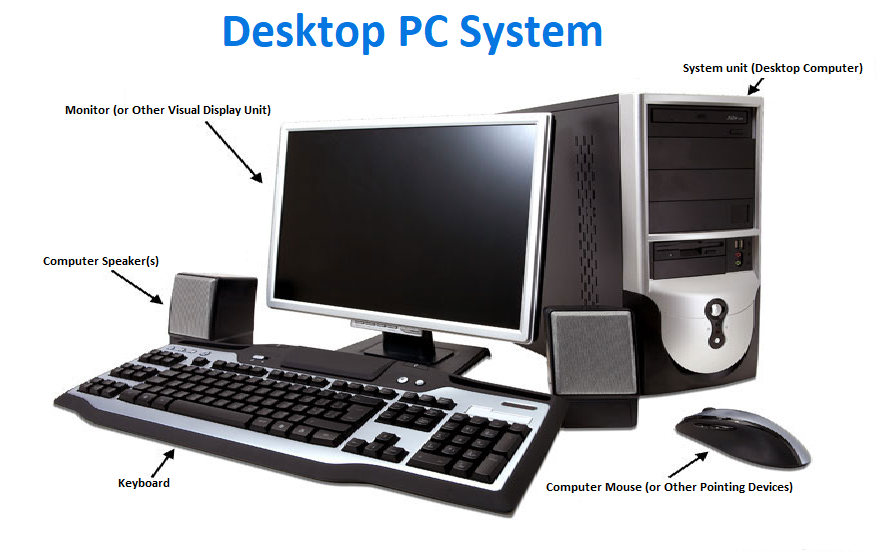
\includegraphics[scale=.2]{gambar/contoh-gambar-miring.png}
    \caption{Komputer}
    \label{fig:komputer}
\end{figure}


\section{Program}
Untuk melampirkan potongan program dapat menggunakan listing, sebagai contoh

\begin{lstlisting}[language=Python,caption={Program perhitungan bilangan prima}, label={lst:bilanganprima}]
import numpy as np

def incmatrix(genl1,genl2):
    m = len(genl1)
    n = len(genl2)
    M = None #to become the incidence matrix
    VT = np.zeros((n*m,1), int)  #dummy variable

    #compute the bitwise xor matrix
    M1 = bitxormatrix(genl1)
    M2 = np.triu(bitxormatrix(genl2),1)

    for i in range(m-1):
        for j in range(i+1, m):
            [r,c] = np.where(M2 == M1[i,j])
            for k in range(len(r)):
                VT[(i)*n + r[k]] = 1;
                VT[(i)*n + c[k]] = 1;
                VT[(j)*n + r[k]] = 1;
                VT[(j)*n + c[k]] = 1;

                if M is None:
                    M = np.copy(VT)
                else:
                    M = np.concatenate((M, VT), 1)

                VT = np.zeros((n*m,1), int)

    return M
\end{lstlisting}



% Baris ini digunakan untuk membantu dalam melakukan sitasi
% Karena diapit dengan comment, maka baris ini akan diabaikan
% oleh compiler LaTeX.
\begin{comment}
\bibliography{daftar-pustaka}
\end{comment}


% Bab 4 hasil dan pembahasan
\chapter{HASIL DAN PEMBAHASAN}

\section{Isi Bab Hasil dan Pembahasan}
\blindtext

\section{Melampirkan Tabel}
\blindtext \ref{table:nilai}.

\begin{table}[H]
\centering
\caption{Parameter kelulusan tugas akhir}
\begin{tabular}{ clc }
\hline
\textbf{No.} & \textbf{Parameter } & \textbf{Nilai} \\
\hline
1. & Penulisan & A \\
2. & Penulisan & A \\
\hline
\end{tabular}
\label{table:nilai}
\end{table}


%Berikut adalah contoh tabel yang dicetak secara horizontal
%gunakan package longtable
%Dapat dibuat dulu di https://www.tablesgenerator.com/ lalu dipindah
\begin{landscape}
\scriptsize
\begin{longtable}{p{3.5cm}cllllll}
\caption{Contoh Tabel Mendatar yang Panjang dan Lebar}\\
\hline
\textbf{Provinsi} & \textbf{Kode Wilayah} & \textbf{Singkatan Umum} & \textbf{ISO} & \textbf{Pulau} & \textbf{Ibu Kota} & \textbf{Gubernur} \\ \hline
\endfirsthead

\multicolumn{4}{l}{\bfseries \tablename\ \thetable{} -- Lanjutan dari halaman sebelumnya}\\
% \begin{center}
% % {{\bfseries \tablename\ \thetable{} -- Lanjutan dari halaman sebelumnya}} \\
% \end{center}
\hline
\textbf{Provinsi} & \textbf{Kode Wilayah} & \textbf{Singkatan Umum} & \textbf{ISO} & \textbf{Pulau} & \textbf{Ibu Kota} & \textbf{Gubernur} \\ \hline

\endhead

\hline
\endfoot

\endlastfoot



Aceh & 11 & Aceh & ID-AC & Sumatera & Banda Aceh & Achmad Marzuki \\
Sumatera Utara & 12 & Sumut & ID-SU & Sumatera & Medan & Edy Rahmayadi \\
Sumatera Barat & 13 & Sumbar & ID-SB & Sumatera & Padang & Mahyeldi Ansharullah \\
Riau & 14 & Riau & ID-RI & Sumatera & Pekanbaru & Syamsuar \\
Jambi & 15 & Jambi & ID-JA & Sumatera & Jambi & Al Haris \\
Sumatera Selatan & 16 & Sumsel & ID-SS & Sumatera & Palembang & Herman Deru \\
Bengkulu & 17 & Bengkulu & ID-BE & Sumatera & Bengkulu & Rohidin Mersyah \\
Lampung & 18 & Lampung & ID-LA & Sumatera & Bandar Lampung & Arinal Djunaidi \\
Kepulauan Bangka Belitung & 19 & Babel & ID-BB & Sumatera & Pangkalpinang & Ridwan Djamaluddin \\
Kepulauan Riau & 21 & Kepri & ID-KR & Sumatera & Tanjungpinang & Ansar Ahmad \\
Daerah Khusus Ibukota Jakarta & 31 & DKI Jakarta & ID-JK & Jawa & Tidak ada & Heru Budi Hartono \\
Jawa Barat & 32 & Jabar & ID-JB & Jawa & Bandung & Ridwan Kamil \\
Jawa Tengah & 33 & Jateng & ID-JT & Jawa & Semarang & Ganjar Pranowo \\
Daerah Istimewa Yogyakarta & 34 & DIY & ID-YO & Jawa & Yogyakarta & Hamengkubuwana X \\
Jawa Timur & 35 & Jatim & ID-JI & Jawa & Surabaya & Khofifah Indar Parawansa \\
Banten & 36 & Banten & ID-BT & Jawa & Serang & Al Muktabar \\
Bali & 51 & Bali & ID-BA & Nusa Tenggara & Denpasar & I Wayan Koster \\
Nusa Tenggara Barat & 52 & NTB & ID-NB & Nusa Tenggara & Mataram & Zulkieflimansyah \\
Nusa Tenggara Timur & 53 & NTT & ID-NT & Nusa Tenggara & Kupang & Viktor Laiskodat \\

Kalimantan Barat & 61 & Kalbar & ID-KB & Kalimantan & Pontianak & Sutarmidji \\
Kalimantan Tengah & 62 & Kalteng & ID-KT & Kalimantan & Palangka Raya & Sugianto Sabran \\
Kalimantan Selatan & 63 & Kalsel & ID-KS & Kalimantan & Banjarbaru & Sahbirin Noor \\
Kalimantan Timur & 64 & Kaltim & ID-KI & Kalimantan & Samarinda & Isran Noor \\
Kalimantan Utara & 65 & Kaltara & ID-KU & Kalimantan & Tanjung Selor & Zainal Arifin Paliwang \\
Sulawesi Utara & 71 & Sulut & ID-SA & Sulawesi & Manado & Olly Dondokambey \\
Sulawesi Tengah & 72 & Sulteng & ID-ST & Sulawesi & Palu & Rusdy Mastura \\
Sulawesi Selatan & 73 & Sulsel & ID-SN & Sulawesi & Makassar & Andi Sudirman Sulaiman \\
Sulawesi Tenggara & 74 & Sultra & ID-SG & Sulawesi & Kendari & Ali Mazi \\
Gorontalo & 75 & Gorontalo & ID-GO & Sulawesi & Gorontalo & Hamka Hendra Noer \\
Sulawesi Barat & 76 & Sulbar & ID-SR & Sulawesi & Mamuju & Akmal Malik \\
Maluku & 81 & Maluku & ID-MA & Maluku & Ambon & Murad Ismail \\
Maluku Utara & 82 & Malut & ID-MU & Maluku & Sofifi & Abdul Ghani Kasuba \\
Papua & 91 & Papua & ID-PA & Papua & Jayapura & Lukas Enembe \\
Papua Barat & 92 & Pabar & ID-PB & Papua & Manokwari & Paulus Waterpauw \\
Papua Selatan & 93 & Pasel & — & Papua & Merauke & Apolo Safanpo \\
Papua Tengah & 94 & Papteng & — & Papua & Nabire & Ribka Haluk \\
Papua Pegunungan & 95 & Papeg & — & Papua & Wamena & Nikolaus Kondomo \\
Papua Barat Daya & 96 & PBD & — & Papua & Sorong1 & — \\ \hline
\label{table:tabelpanjanglebar}
\end{longtable}
\end{landscape}


		\subsection{Subsubbab 2 2}
		\blindtext

	\section{Subab 3}
	\blindtext \ref{fig:komputer}

\begin{equation}
    x+2 = 159
\end{equation}
\blindtext

%Berikut adalah contoh gambar yang dicetak secara horizontal
\begin{landscape}
   \begin{figure}[t]
        \centering
        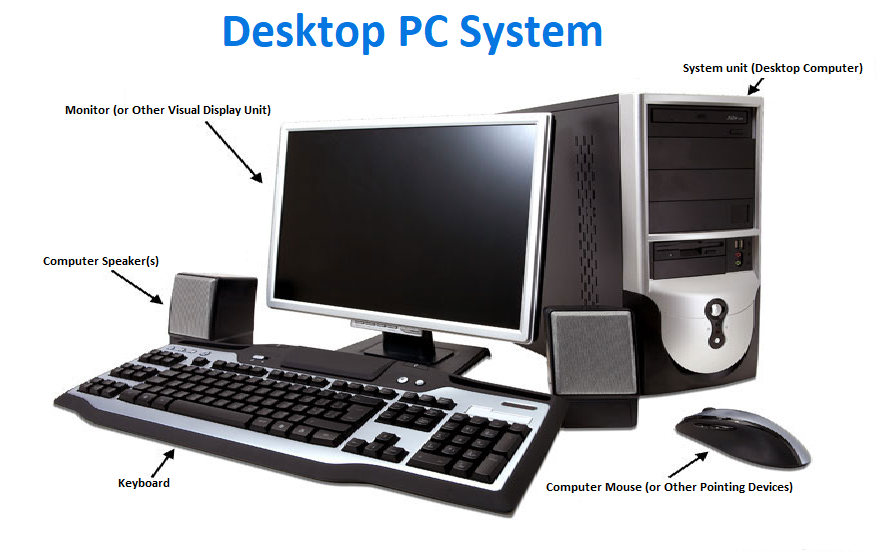
\includegraphics[width=18cm, height=12cm]{gambar/contoh-gambar-miring.png}
        \caption{Contoh Gambar Komputer}
        \label{fig:komputer}
    \end{figure}
\end{landscape}



% Bab 5 penutup
\chapter{KESIMPULAN DAN SARAN}

\section{Kesimpulan}
\noindent Berdasarkan hasil analisis dan pengujian fungsional aplikasi ini, didapat kesimpulan sebagai berikut:

\begin{enumerate}
	\item Lorem ipsum is a pseudo-Latin text used in web design, typography, layout, and printing in place of English to emphasise design elements over content.

	\item It's also called placeholder (or filler) text. It's a convenient tool for mock-ups.

	\item It helps to outline the visual elements of a document or presentation, eg typography, font, or layout. Lorem ipsum is mostly a part of a Latin text by the classical author and philospher Cicero.

	\item Its words and letters have been changed by addition or removal, so to deliberately render its content nonsensical; it's not genuine, correct, or comprehensible Latin anymore.
\end{enumerate}


\section{Saran}
\noindent Hal-hal penting terkait pelaksanaan penelitian yang perlu diperhatikan kedepannya adalah
\begin{enumerate}
	\item Lorem ipsum is a pseudo-Latin text used in web design, typography, layout, and printing in place of English to emphasise design elements over content.

	\item It's also called placeholder (or filler) text. It's a convenient tool for mock-ups.

	\item It helps to outline the visual elements of a document or presentation, eg typography, font, or layout. Lorem ipsum is mostly a part of a Latin text by the classical author and philospher Cicero.

	\item Its words and letters have been changed by addition or removal, so to deliberately render its content nonsensical; it's not genuine, correct, or comprehensible Latin anymore.
\end{enumerate}


% Baris ini digunakan untuk membantu dalam melakukan sitasi
% Karena diapit dengan comment, maka baris ini akan diabaikan
% oleh compiler LaTeX.
\begin{comment}
\bibliography{daftar-pustaka}
\end{comment}


% Daftar Pustaka
\phantomsection%<---
\addcontentsline{toc}{chapter}{DAFTAR PUSTAKA}
\sloppy
\printbibliography

% Halaman lampiran di tengah
\newpage
\phantomsection%<---
\addcontentsline{toc}{chapter}{LAMPIRAN}
\begin{center}
    \thispagestyle{empty}
    \vspace*{\fill}
    \noindent \Huge{LAMPIRAN}
\vspace*{\fill}
\end{center}


% Lampiran
\begin{appendix}
\phantomsection%<---
\chapter{Rencana Pengamatan}
Lampiran ini berisikan rencana pengamatan dalam bentuk \textit{finding chart} dan catatan pengamatan berupa \textit{logbook}.


\chapter{Hasil Pengamatan} \label{lampiranD}
Lampiran hasil pengamatan berisikan dengan \textit{logbook} selama pengamatan, citra objek, keluaran algoritma, skrip pengolahan data dengan Python, dan dokumentasi selama pengamatan.
    \section{\textit{Logbook} Pengamatan}
     Lorem ipsum dolor sit amet, consectetur adipiscing elit, sed do eiusmod tempor incididunt ut labore et dolore magna aliqua. Ut enim ad minim veniam, quis nostrud exercitation ullamco laboris nisi ut aliquip ex ea commodo consequat. Duis aute irure dolor in reprehenderit in voluptate velit esse cillum dolore eu fugiat nulla pariatur. Excepteur sint occaecat cupidatat non proident, sunt in culpa qui officia deserunt mollit anim id est laborum.
    \section{Objek pada Citra Pengamatan}
    Lorem ipsum dolor sit amet, consectetur adipiscing elit, sed do eiusmod tempor incididunt ut labore et dolore magna aliqua. Ut enim ad minim veniam, quis nostrud exercitation ullamco laboris nisi ut aliquip ex ea commodo consequat. Duis aute irure dolor in reprehenderit in voluptate velit esse cillum dolore eu fugiat nulla pariatur. Excepteur sint occaecat cupidatat non proident, sunt in culpa qui officia deserunt mollit anim id est laborum

    \section{Dokumentasi Pengamatan}
  Lorem ipsum dolor sit amet, consectetur adipiscing elit, sed do eiusmod tempor incididunt ut labore et dolore magna aliqua. Ut enim ad minim veniam, quis nostrud exercitation ullamco laboris nisi ut aliquip ex ea commodo consequat. Duis aute irure dolor in reprehenderit in voluptate velit esse cillum dolore eu fugiat nulla pariatur. Excepteur sint occaecat cupidatat non proident, sunt in culpa qui officia deserunt mollit anim id est laborum

\phantomsection%<---
\chapter{Program} \label{lam:lampiran_a}
\begin{lstlisting}[language=Python]
import numpy as np

def incmatrix(genl1,genl2):
    m = len(genl1)
    n = len(genl2)
    M = None #to become the incidence matrix
    VT = np.zeros((n*m,1), int)  #dummy variable

    #compute the bitwise xor matrix
    M1 = bitxormatrix(genl1)
    M2 = np.triu(bitxormatrix(genl2),1)

    for i in range(m-1):
        for j in range(i+1, m):
            [r,c] = np.where(M2 == M1[i,j])
            for k in range(len(r)):
                VT[(i)*n + r[k]] = 1;
                VT[(i)*n + c[k]] = 1;
                VT[(j)*n + r[k]] = 1;
                VT[(j)*n + c[k]] = 1;

                if M is None:
                    M = np.copy(VT)
                else:
                    M = np.concatenate((M, VT), 1)

                VT = np.zeros((n*m,1), int)

    return M
\end{lstlisting}

\phantomsection%<---
\chapter{Grafik Tambahan} \label{lampiran B}
 Lorem ipsum dolor sit amet, consectetur adipiscing elit, sed do eiusmod tempor incididunt ut labore et dolore magna aliqua. Ut enim ad minim veniam, quis nostrud exercitation ullamco laboris nisi ut aliquip ex ea commodo consequat. Duis aute irure dolor in reprehenderit in voluptate velit esse cillum dolore eu fugiat nulla pariatur. Excepteur sint occaecat cupidatat non proident, sunt in culpa qui officia deserunt mollit anim id est laborum

\end{appendix}

\end{document}